\newpage
\section{Questão 12-30}

\begin{figure}[H]
	\centering
	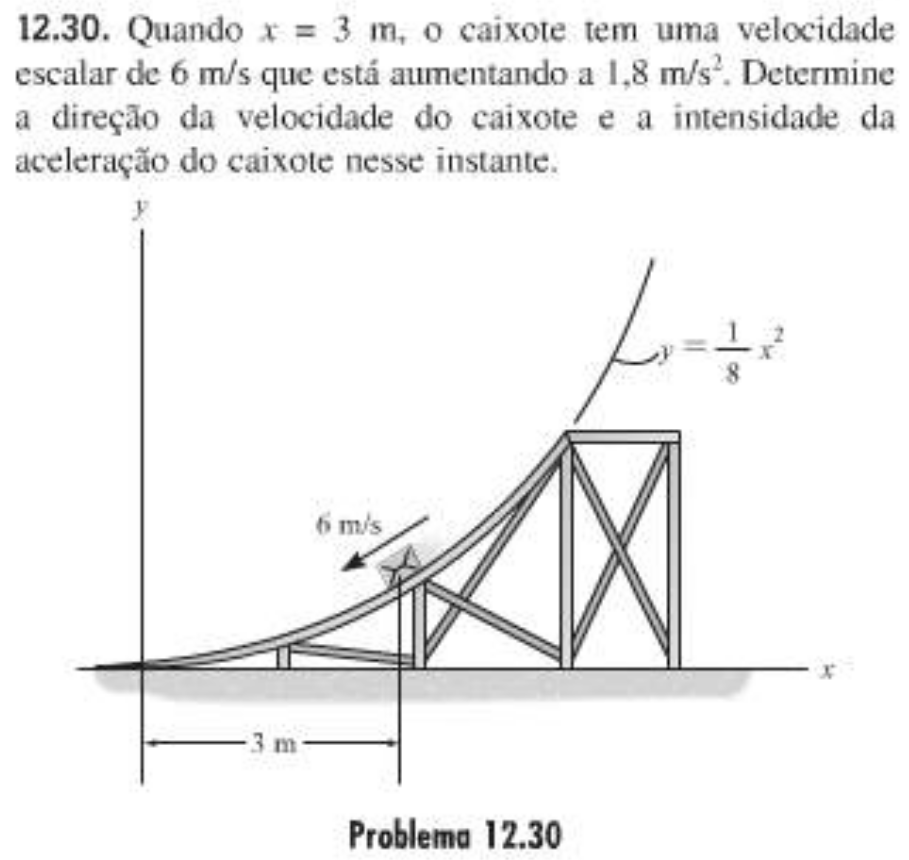
\includegraphics[width=0.7\linewidth]{fundamentais/12-30.png}
	\caption{Comando da questão 12-30}\label{fig:q12-30}
\end{figure}

Nesta questão, analisamos o movimento de uma partícula cuja trajetória é descrita por \(y = \frac{1}{8}x^2\). Sabendo que a velocidade escalar é constante (\(v = 6 \, \text{m/s}\)) e que a aceleração tangencial é \(a_t = 1.8 \, \text{m/s}^2\), determinamos o ângulo de inclinação da trajetória (\(\theta\)), a aceleração normal (\(a_n\)) e a aceleração total (\(a_{\text{total}}\)) no ponto \(x = 3 \, \text{m}\).

\subsection*{Equação da Trajetória}
A equação da trajetória é dada por:
\[
y = \frac{1}{8}x^2.
\]

\subsection*{Derivada da Trajetória e Ângulo de Inclinação}
A inclinação da trajetória é obtida pela derivada de \(y\) em relação a \(x\):
\[
\frac{dy}{dx} = \frac{1}{4}x.
\]

O ângulo de inclinação \(\theta\) é dado por:
\[
\theta = \arctan\left(\frac{dy}{dx}\right).
\]

Substituindo \(x = 3 \, \text{m}\):
\[
\theta = \arctan\left(\frac{1}{4} \cdot 3\right) = \arctan\left(\frac{3}{4}\right).
\]

Convertendo para graus:
\[
\theta \approx 36.87^\circ.
\]

\subsection*{Segunda derivada}
A derivada de segunda ordem, ou segunda derivada de \(y\), é:

\[\frac{d^2y}{dx^2} = \frac{d^2}{dx^2}\left(\frac{x}{4}\right) = \frac{1}{4} \]

\subsection*{Aceleração Normal (\(a_n\))}
A aceleração normal é calculada como:

\[
a_n = \frac{v^2}{\rho}
\]

onde:

\[
\rho = \frac{\left[1 + \left(\frac{dy}{dx}\right)^2 \right]^{(3/2)}}{ 
\left|\frac{d^2y}{dx^2} \right|}
\]


Substituímos \(v = 6 \, \text{m/s}\), \(\frac{dy}{dx} = \frac{1}{4}x\) e \(\frac{d^2y}{dx^2} = \frac{1}{4}\):

\[
a_n = \frac{6^2 \cdot \left|\frac{1}{4}\right|}{\sqrt{\left(1 + \left(\frac{1}{4}x\right)^2\right)^3}}.
\]

Para \(x = 3 \, \text{m}\):
\[
a_n = \frac{6^2 \cdot \left|\frac{1}{4}\right|}{\sqrt{\left(1 + \left(\frac{1}{4} \cdot 3\right)^2\right)^3}} = \frac{9}{\left(\sqrt{1 + \left(\frac{3}{4}\right)^2}\right)^3}.
\]

Simplificando:
\[
a_n \approx 4.608 \, \text{m/s}^2.
\]

\subsection*{Aceleração Total (\(a_{\text{total}}\))}
A aceleração total é a soma vetorial das componentes tangencial e normal:
\[
a_{\text{total}} = \sqrt{a_t^2 + a_n^2}.
\]

Substituímos \(a_t = 1.8 \, \text{m/s}^2\) e \(a_n \approx 8.57 \, \text{m/s}^2\):
\[
a_{\text{total}} = \sqrt{1.8^2 + 4.61^2}.
\]

Simplificando:
\[
a_{\text{total}} \approx 4.948 \, \text{m/s}^2.
\]

\subsection*{Resultados Finais}
\begin{itemize}
    \item Ângulo de inclinação:
    \[
    \theta \approx 36.87^\circ \quad \text{(em \(x = 3 \, \text{m}\))}.
    \]
    \item Aceleração normal:
    \[
    a_n \approx 4.608 \, \text{m/s}^2 \quad \text{(em \(x = 3 \, \text{m}\))}.
    \]
    \item Aceleração total:
    \[
    a_{\text{total}} \approx 4.948 \, \text{m/s}^2 \quad \text{(em \(x = 3 \, \text{m}\))}.
    \]
\end{itemize}
